%----------------------------------------------------------------------------
\chapter{Tervezés}
\label{chp:design}
%----------------------------------------------------------------------------
Ebben a fejezetben bemutatok egy olyan modellt, ami oktatási laborokat tud ábrázolni, illetve definiálok rajta végezhető terítési műveleteket, ezáltal magyarázva a terítési folyamat működését. Végül a megvalósítandó Torrent alapú fájlterítési megoldás felépítését részletezem.

%----------------------------------------------------------------------------
\section{Terítési feladat modellezése}
%----------------------------------------------------------------------------
\label{design_model}

Egy modell megalkotásakor érdemes először a feladatot könnyebben kezelhető részekre bontani, a mi esetünkben ez a modell három részre szedését eredményezi, ami \aref{fig:designmodelparts}-es ábra illusztrál. A három rész a laborban levő számítógépek (Computer), virtuális gépek (VirtualMachine) és a lehetséges terítési célállapotok (Lab).

\begin{figure}[ht]
	\centering
	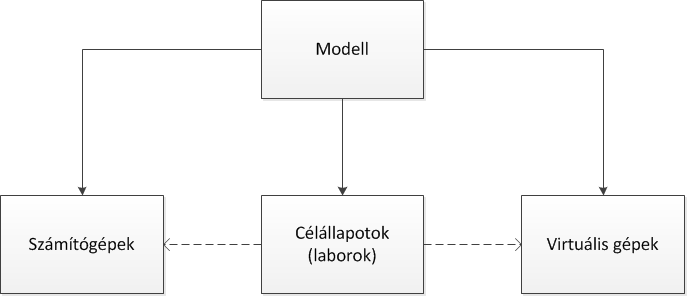
\includegraphics[width=100mm, keepaspectratio]{figures/design_modelparts.png}
	\caption{Labor modelljének három része.}
	\label{fig:designmodelparts}
\end{figure}

Vegyük először a virtuális gépek modelljét(\ref{fig:designvm}-es ábra)! A terítendő VM-ek azon tulajdonságainak kell a modellben megjelennie, amelyekre a fájlterítés során szükségünk lesz, ezek pedig a VM neve, az őt tartalmazó fájl elérési útvonala és használatának követelményei. Utóbbinál a rendelkezésre álló memória mennyiségét, rendelkezésre álló szabad tárterület méretét és a rendszer architektúráját kell feltüntetnünk, mert csak ezek befolyásolják a gépekkel való kompatibilitást. Érdemes megkülönböztetni a Vagrant által készíttetendő VM-eket, mert róluk extra információkat kell eltárolnunk (VagrantVM a VirtualMachine leszármazottja lesz). Jobban átlátható modellt kapunk, ha a követelmények tárolását ``kiszervezzük'', és a Requirements osztályban tároljuk ahelyett, hogy minden VirtualMachine-nél attribútumként vennénk fel. Érdemes azt is eltárolnunk, hogy egy VM melyik számítógépen van, sok, a modellen értelmezhető művelet futási idejét tudjuk felgyorsítani vele, például ha egy adott VM-et szeretnénk majd törölni a gépekről, akkor nem kell az összesen végigmennünk, hanem közvetlen törölhetjük azokról, amelyiken rajta van.

\begin{figure}[ht]
	\centering
	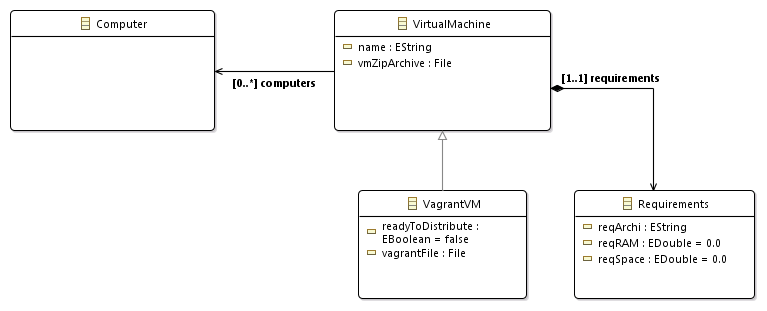
\includegraphics[width=130mm, keepaspectratio]{figures/design_vm.png}
	\caption{Labormodell - virtuális gépek}
	\label{fig:designvm}
\end{figure}

Hasonló megfontolásokkal készíthetjük el a számítógépek modelljét (\ref{fig:designcomputers}-as ábra), a számunkra fontos adatok itt a számítógép neve, elérhetősége és azon tulajdonságai, amik egy VM-el való kompatibilitást meghatároznak. Azt is el kell tárolnunk értelemszerűen, hogy adott számítógépen melyik virtuális gépek vannak már rajta. A számítógép elérhetőségeihez kapcsolódó attribútumokat nem csak azért tettük ConnectionInfo objektumokba, mint az előbbieknél a Requirements-be, hanem mert érzékeny adatokat is tárol (felhasználónév + jelszó).

\begin{figure}[ht]
	\centering
	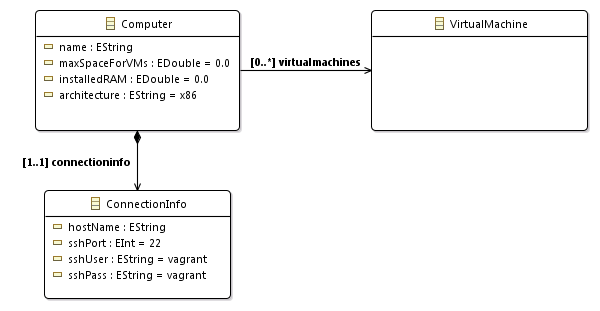
\includegraphics[width=110mm, keepaspectratio]{figures/design_computer.png}
	\caption{Labormodell - számítógépek}
	\label{fig:designcomputers}
\end{figure}

Az utolsó modellezendő dolog a terítés végállapota (\ref{fig:designlab}-es ábra), ami egy tanórához tartozó labor felépítését tartalmazza, vagyis az összes szükséges számítógép $\rightarrow$ virtuális gép hozzárendelést. Ezt modell szinten úgy tudjuk leírni, hogy a végállapot tartalmaz minden számítógéphez egy ComputerConfig-ot, ami adott számítógépekre terítendő virtuális gépek listáját tartalmazza, és persze hivatkozik a konkrét számítógépre is.

\begin{figure}[h!]
	\centering
	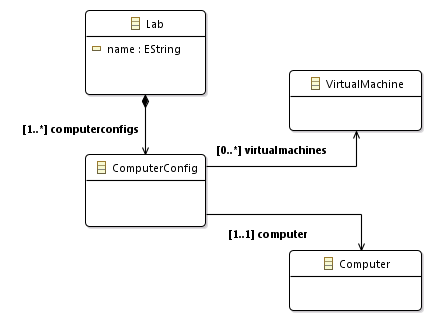
\includegraphics[width=100mm, keepaspectratio]{figures/design_lab.png}
	\caption{Labormodell - laborok(célállapotok)}
	\label{fig:designlab}
\end{figure}

Az előbb leírt modellrészletek összefogásához még szükségünk egy olyan elemre, ami mindhárom részt összefogja (\ref{fig:designmodelroot}-ös ábra). A LabSystem lesz a modell gyökéreleme, ez fogja tárolni a laborunkban található össze számítógépet, virtuális gépet és az összes felvett terítési végállapotot. Azt is itt tároljuk, hogy melyik számítógépet választjuk a Torrent alapú terítés során sedd-nek.

\begin{figure}[h!]
	\centering
	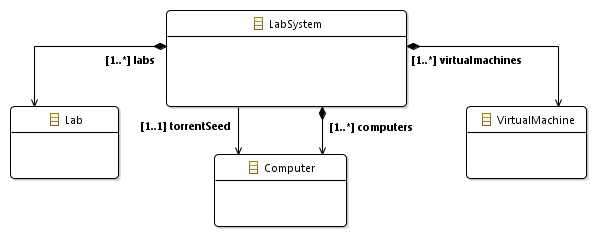
\includegraphics[width=130mm, keepaspectratio]{figures/design_modelroot.png}
	\caption{Labormodell - gyökérelem}
	\label{fig:designmodelroot}
\end{figure}

%----------------------------------------------------------------------------
\section{Terítési műveletek a modellen}
%----------------------------------------------------------------------------
\label{distrops}

Annak a megtervezésére, hogy egy fájlterítési folyamat hogyan zajlik érdemes azt kisebb darabokba vágni, azt definiálni egyszerű műveletekkel.
Az előbbi fejezetben ismertetett modellre definiálok itt terítési műveleteket, és megkísérlem leírni segítségükkel az egész fájlterítési folyamatot.
Az egyszerű műveleteket a következő formátumban fogom definiálni: METHOD\_NAME(parameter1\_name: parameter1\_type, parameter2\_name\ldots).

A modellen értelmezett terítési műveletek:

\begin{itemize}
  \item REMOVE\_DUPLICATES(goal: Lab, resources: LabSystem): Ez a művelet a paraméterei között különbséget képez, vagyis a Lab-ből kiszedi azokat a (Computer, VirtualMachine) párokat, amik a LabSystem-ben már szerepelnek. Ennek az a célja, hogy a terítendő VM-ek közül kiszűrje azokat, amelyek már ott vannak, ahova terítenénk őket.
  \item DELETE(to\_be\_deleted\_vm : VirtualMachine, from\_pcs: List<Computer>): Ezzel a művelettel törölhetjük a második paraméter Computer-eket tartalmazó lista összes eleméről az adott virtuális gépet.
  \item ISCOMPATIBLE(pc: Computer, vm: VirtualMachine): Arra a kérdésre válaszol, hogy adot VM kompatibilis-e a Computer-rel. Ellenőrzi az architektúrák megfelelését, a memória és a szabad lemezterület méretét.
  \item UPLOAD(vm: VirtualMachine, pc: Computer): Feltölti a VM-et a Computer-re, vagyis hozzáadja annak a \code{virtualmachines} listájához. 
\end{itemize}

% \begin{program}
% \mbox{A fast exponentiation procedure:}
% \BEGIN \\ %
%   \FOR i:=1 \TO 10 \STEP 1 \DO
%      |expt|(2,i); \\ |newline|() \OD %
% \rcomment{This text will be set flush to the right margin}
% \WHERE
% \PROC |expt|(x,n) \BODY
%           z:=1;
%           \DO \IF n=0 \THEN \EXIT \FI;
%              \DO \IF |odd|(n) \THEN \EXIT \FI;
% \COMMENT{This is a comment statement};
%                 n:=n/2; x:=x*x \OD;
%              \{ n>0 \};
%              n:=n-1; z:=z*x \OD;
%           |print|(z) \ENDPROC
% \END
% \end{program}

Az előbbiek segítségével már felírható a DISTRIBUTION(goal: Lab, resources: LabSystem) művelet:

\code{DISTRIBUTION(goal: Lab, resources: LabSystem):}\\
\indent \code{goal\_no\_duplicates = REMOVE\_DUPLICATES(goal, resources)}\\
\indent \indent \code{FOR all ComputerConfigs in goal\_no\_duplicates}\\
\indent \indent \indent	\code{FOR all VirtualMachines in ComputerConfig.Virtualmachines}\\
\indent \indent \indent	\code{IF(ISCOMPATIBLE(ComputerConfig.Computer, VirtualMachine))}\\
\indent \indent \indent \indent	\code{THEN UPLOAD(VirtualMachine, ComputerConfig.Computer)}


%----------------------------------------------------------------------------
\section{P2P-alapú fájlterítés működése}
%----------------------------------------------------------------------------
\label{design_apparchi}

Az általam készített fájlterítési megoldás a következőképpen működik:

\begin{enumerate}
  \item Beolvassa a labor \ref{design_model}-es fejezetben ismertetett felépítésű modelljét
  \item Lefuttatja a modellen a \ref{distrops}-es fejezetből a TERÍTÉS nevű műveletet
\end{enumerate}

A TERÍTÉS művelet megvalósítása a gyakorlatban úgy fog kinézni, hogy az összes terítendő VM-et felmásoljuk a seed-nek kijelölt gépre, ott torrent fájlokat hozunk létre hozzájuk, és ezeket küldjük a célgépeknek (és persze távolról elindítjuk a torrentklienseiket is). A terítési folyamat státuszát bizonyos időközönként lekérjük az összes swarm-beli gépről. Ezt az egész folyamatot ábrázolja \aref{fig:designoverview}-os ábra.

\begin{figure}[ht]
	\centering
	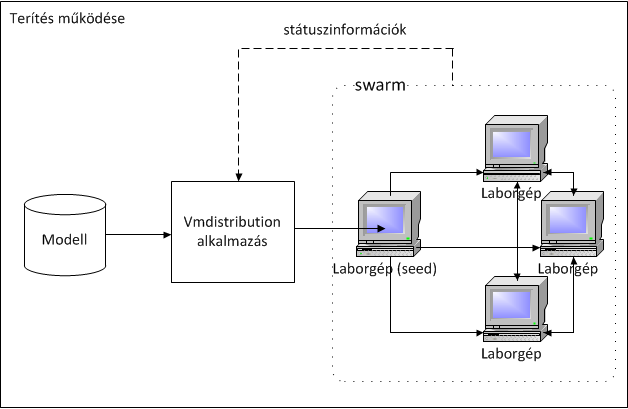
\includegraphics[width=115mm, keepaspectratio]{figures/design_overview.png}
	\caption{Új terítési megoldás működésének folyamata}
	\label{fig:designoverview}
\end{figure}

\Aref{fig:designprotocols}-es ábra pedig azt mutatja be, hogy a terítés egyes szereplői milyen protokollokat használnak az egymással való kommunikációra.

Az egyes használt protokollok rövid leírása:

\begin{itemize}
  \item \textbf{SSH}\cite{ylonen2006secure}\textbf{:} Lehetővé teszi távoli gépekre a bejelentkezést és parancsok futtatását.
  \item \textbf{SCP}\cite{pechanec2007scp}\textbf{:} SSH-n keresztüli fájlátvitelt  valósít meg.
  \item \textbf{XMLRPC:} Bizonyos alkalmazásokkal való távoli kommunikációra használhatjuk, jelen esetben a torrentkliensektől ezzel kérjük le a letöltések aktuális állapotát. Bővebb leírásért lásd \aref{sect:p2p}-es fejezetet.
  \item \textbf{Bittorrent:} P2P fájlátviteli protokoll, részletesebb leírásáért lásd \aref{sect:p2p}-es fejezetet.
\end{itemize}

\begin{figure}[ht]
	\centering
	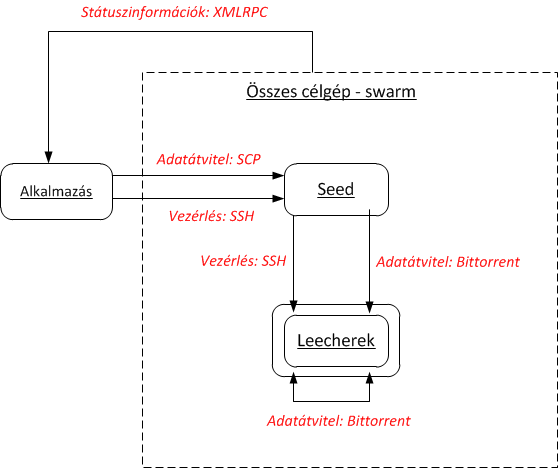
\includegraphics[width=90mm, keepaspectratio]{figures/design_protocols.png}
	\caption{Terítési folyamat egyes szereplői között használt kommunikációs protokollok}
	\label{fig:designprotocols}
\end{figure}

